%% \begin{slide}{XAFS Theory: X-ray Absorption by a Free Atom}
\begin{slide}{X-ray Polarization}

  A synchrotron is highly polarized ( $ > 99.9\% $) in the horizontal
  plane.

\begin{columns}[T]
\begin{column}{58mm}

    \vmm

    A photo-electron from a $K$ shell goes as a $p$ orbital ($\cos^2\theta
    $), mostly in the horizontal plane.
    \vmm

    It {\RedEmph{never}} sees atoms in the vertical (y) plane or along the
    beam direction (z).

  \end{column}
  \begin{column}{52mm}
    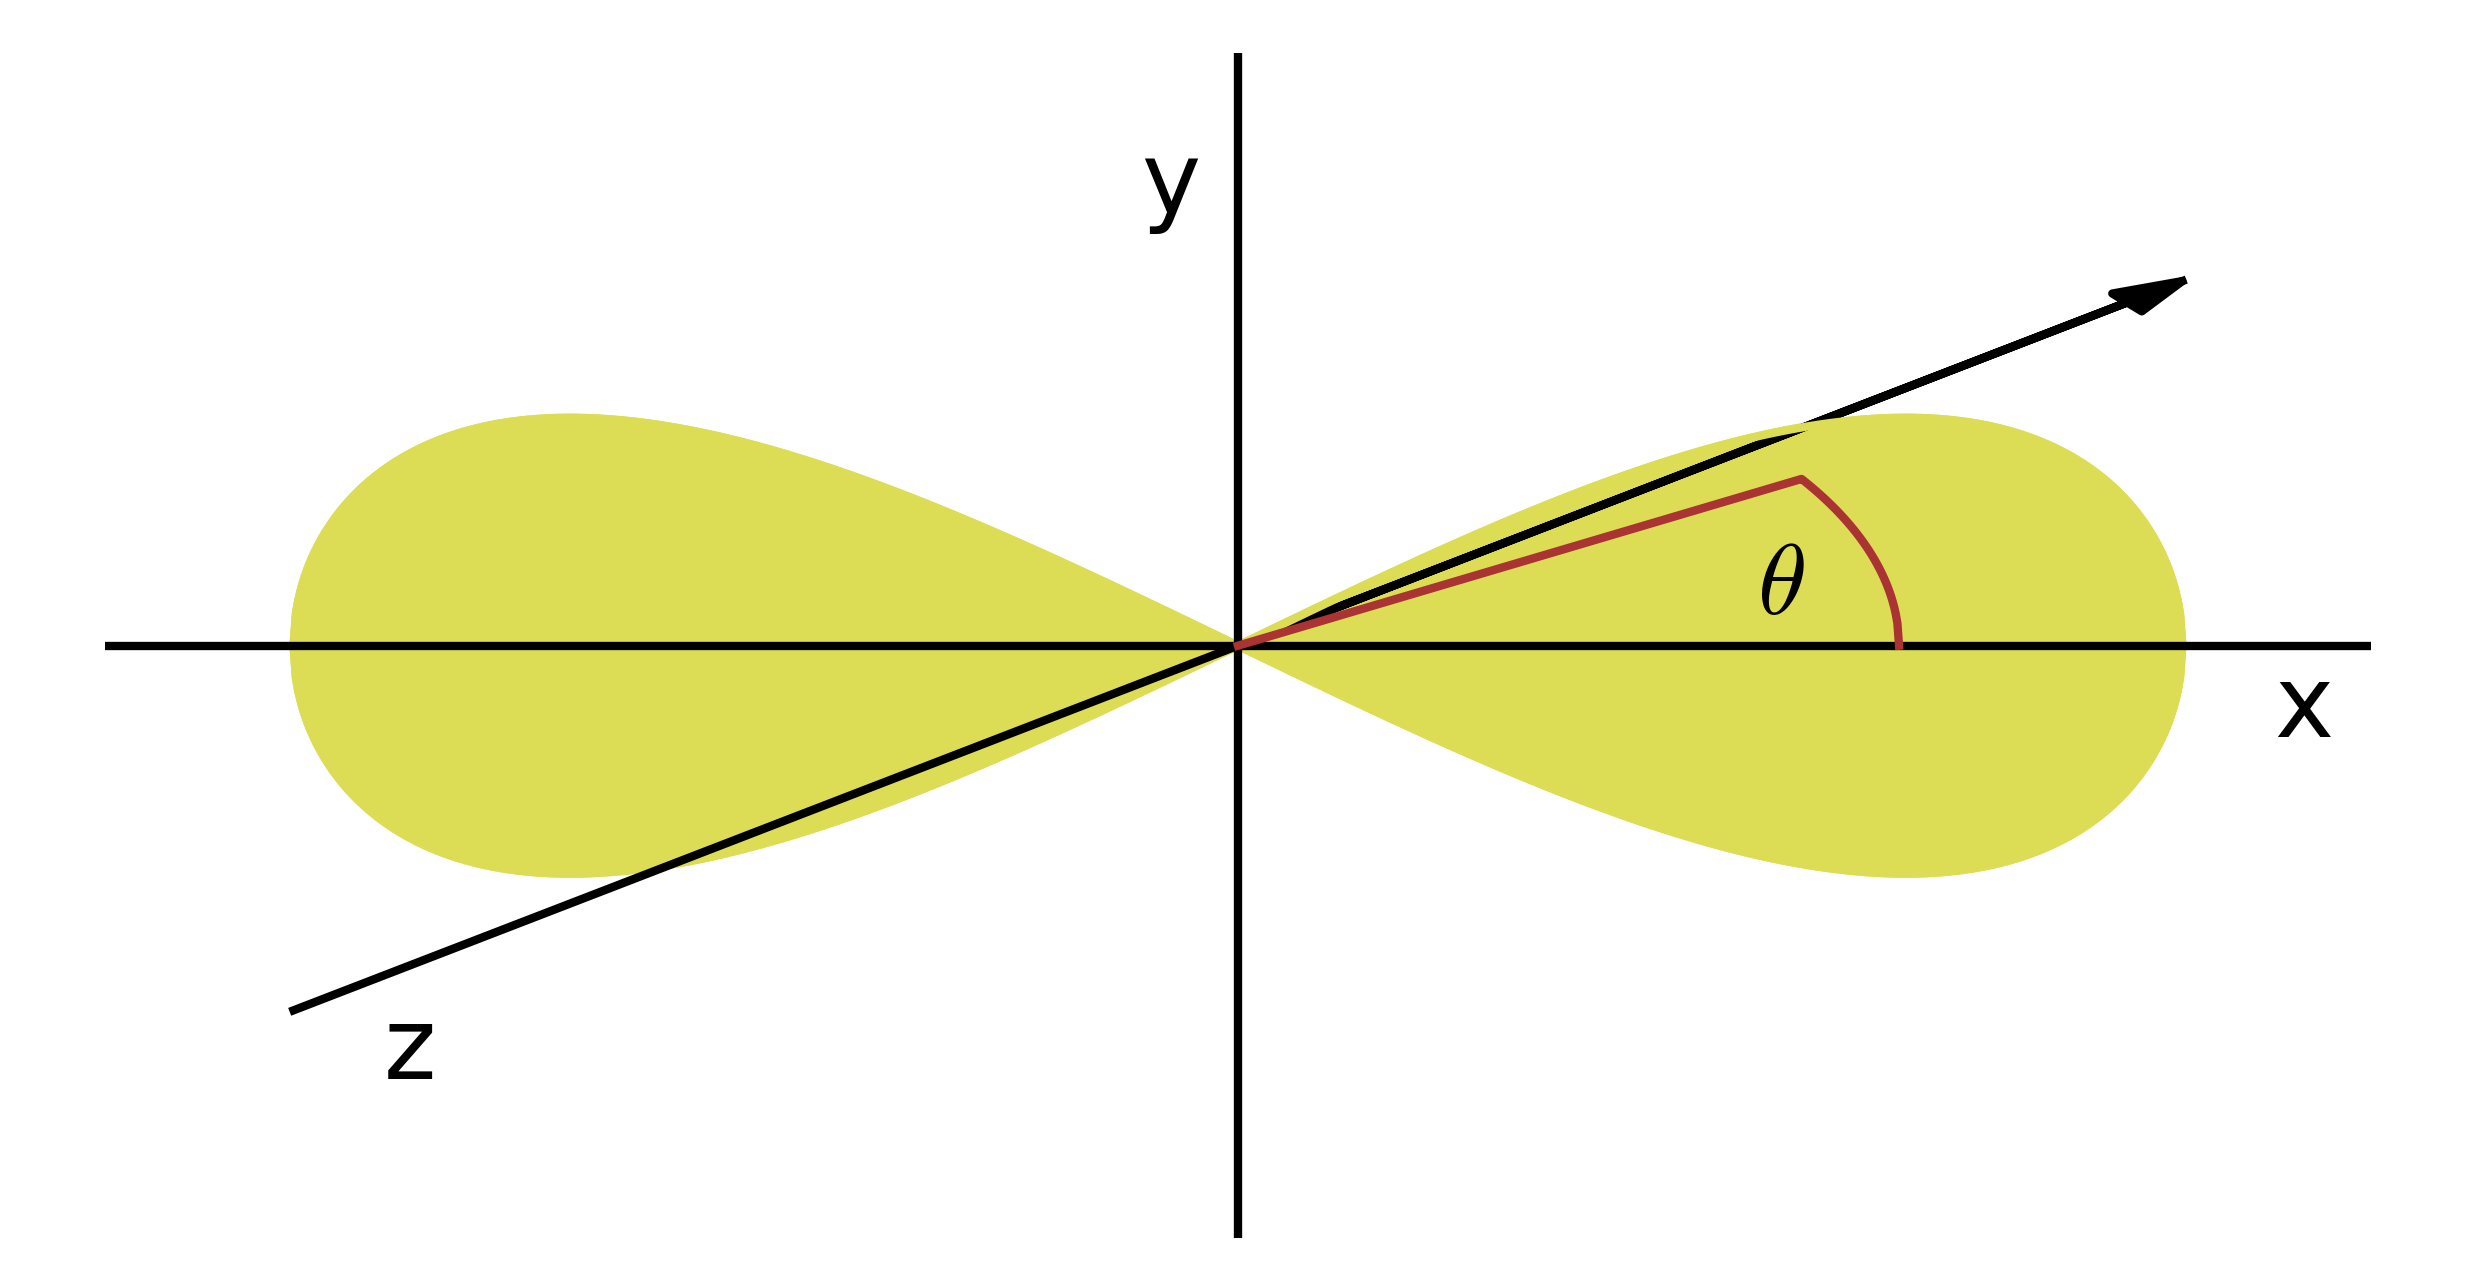
\includegraphics[width=50mm]{figs/theory/dipole}
  \end{column}
  \end{columns}

  \begin{cenpage}{110mm}

  For anisotropic systems (surfaces, non-cubic crystals, \ldots) this can
  be important:  It can be either confounding or useful!

  \vmm\vmm

  \begin{columns}
    \begin{column}{20mm}
      \wgraph{18mm}{xtals/YBCO}

     \end{column}
     \begin{column}{75mm}
       Anistropy of the {\RedEmph{crystal}} doesn't really matter
       -- anisotropy in the {\RedEmph{local structure}} does.

       \vmm

       A sorbed ion on a surface, or ion intercalated in a layered
       material, may show very strong polarization dependence.

     \end{column}
 \end{columns}

 \end{cenpage}

\vfill
\end{slide}
